\apendice{Especificación de diseño}

\section{Introducción}
En este anexo será descrito el diseño, el cual ha sido llevado a cabo en el desarrollo de la plataforma buscando los objetivos y funcionalidades descritos anteriormente. En concreto, viendo el diseño de datos, el diseño procedimental y el diseño arquitectónico.

\section{Diseño de datos}
Las entidades definidas para el funcionamiento de la plataforma y presentes en base de datos son las siguientes:

\begin{itemize}
\item Usuario (User): correspondiente a los usuarios del sistema los cuales pueden ser de tipo profesor o de tipo alumno. Cuentan con identificador, nombre, nombre de usuario, contraseña, campo de control de tipo de usuario y campo de control de primer inicio de sesión.

\item Curso (Course): correspondiente a los cursos del sistema. Cuenta con identificador, identificador del usuario profesor al que pertenece el curso, nombre y descripción 

\item Sección (Section): correspondiente a las secciones de los cursos. Cuenta con identificador, identificador del curso al que pertenece, nombre, nombre del archivo de contenido de la sección y nombre de la tarea de la sección.

\item Calificación (Calification): Correspondiente a las calificaciones de los alumnos. Cuenta con el identificador del estudiante al que pertenece, identificador de la sección a la que pertenece, nombre de la tarea y el valor obtenido.

\item Miembros del curso(Course Members): encargada de guardar las relaciones entre los cursos y los alumnos pertenecientes a estos. Cuenta con el identificador del curso y el del estudiante registrado en el curso.

\item Sección sin publicar (Unreleased Section): correspondiente a secciones no publicadas dedicadas a la creación de tareas de forma manual por los profesores desde la plataforma. Cuenta con identificador, identificador del profesor al que pertenecen, identificador del curso al que pertenecen, nombre, nombre del archivo de contenido de la sección y nombre de la tarea de la sección.


\subsubsection{Diagrama E/R}
\begin{figure}[H]
    \centering
    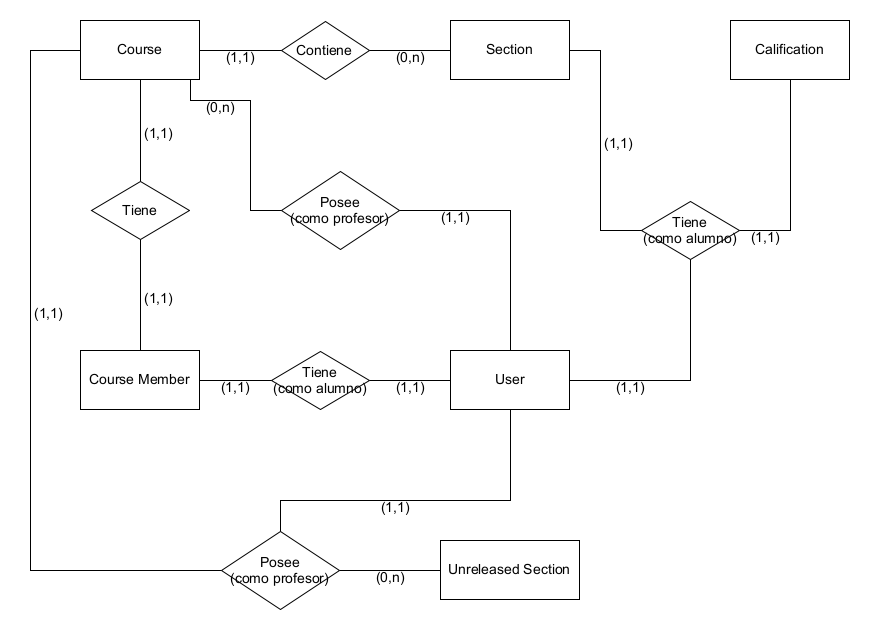
\includegraphics[width=\textwidth]{img/imgs-memoria/BD_DiagramaER.png}
    \caption{Diagrama E/R}
\end{figure}


\subsubsection{Diagrama Relacional}
\begin{figure}[H]
    \centering
    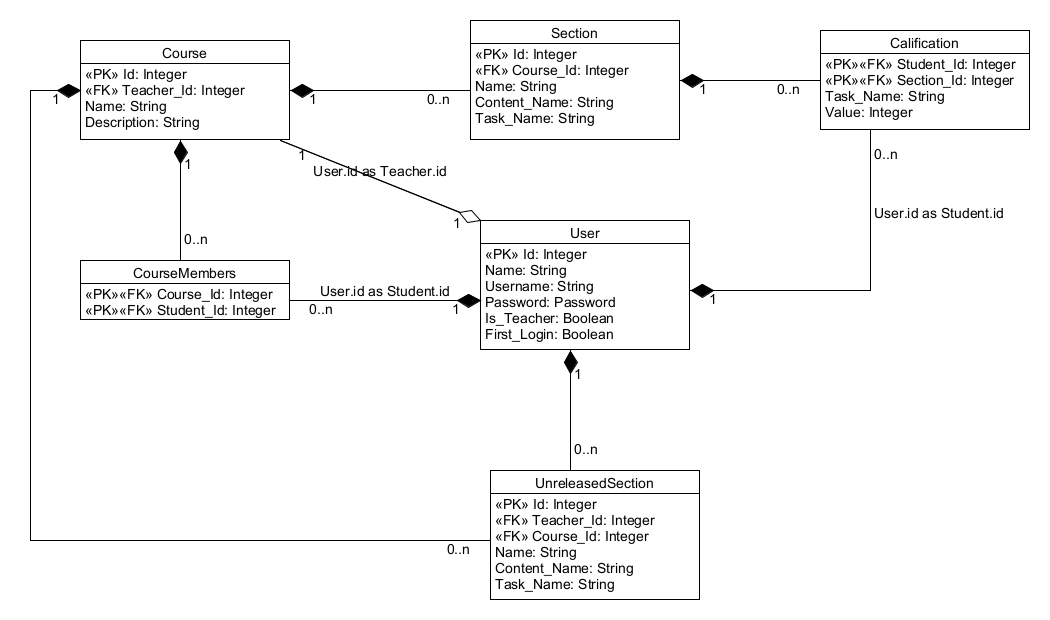
\includegraphics[width=\textwidth]{img/imgs-memoria/BD_DiagramaRelacional.png}
    \caption{Diagrama relacional}
\end{figure}


\end{itemize}

\section{Diseño procedimental}
En esta sección se van a recoger los aspectos más relevantes del diseño procedimental mediante la representación de los diagramas de secuencias de las funcionalidades fundamentales de la plataforma.

El siguiente diagrama de secuencias representa la realización y muestreo de consultas de datos por parte de un usuario las cuales son realizadas mediante SQLAlchemy, herramienta mencionada con anterioridad. En este tipo de consultas se encuentran la consulta de calificaciones por parte de un profesor o alumno, la consulta de alumnos por parte de un profesor, el muestreo de cursos y el muestreo de contenidos (secciones) de un curso:

\begin{figure}[H]
    \centering
    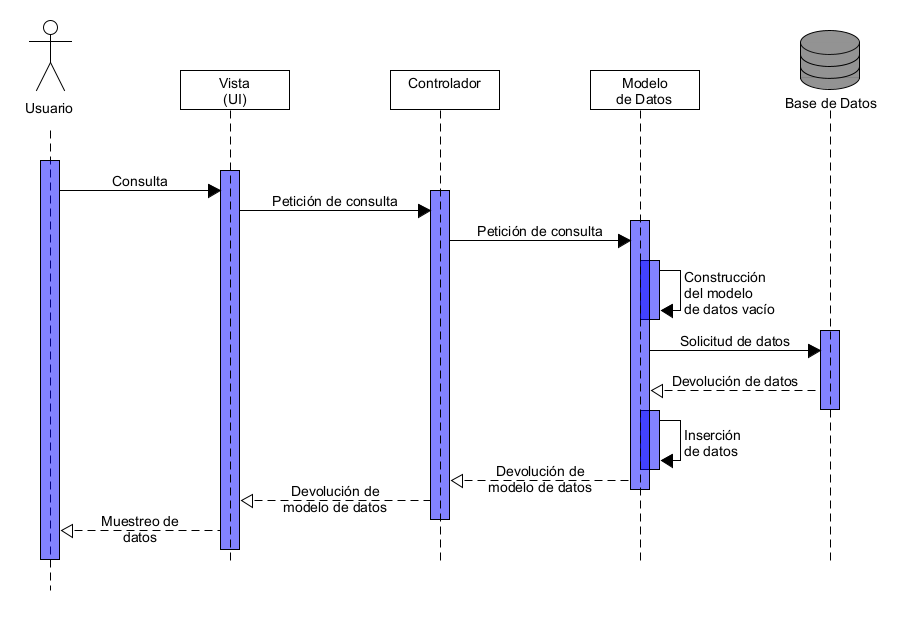
\includegraphics[width=\textwidth]{img/imgs-memoria/Secuencias_Consulta.png}
    \caption{Diagrama de secuencias de una consulta}
\end{figure}

El siguiente diagrama de secuencias representa la inserción o eliminación de datos por parte de un usuario, acciones también realizadas gracias a SQLAlchemy. En este tipo de acciones se encuentran la adición de alumnos, cursos y secciones por parte de un profesor, generación de calificaciones tras enviar una tarea por parte de un alumno y la emiminación de todos los tipos de datos anteriores:

\begin{figure}[H]
    \hspace*{-1.5cm} 
    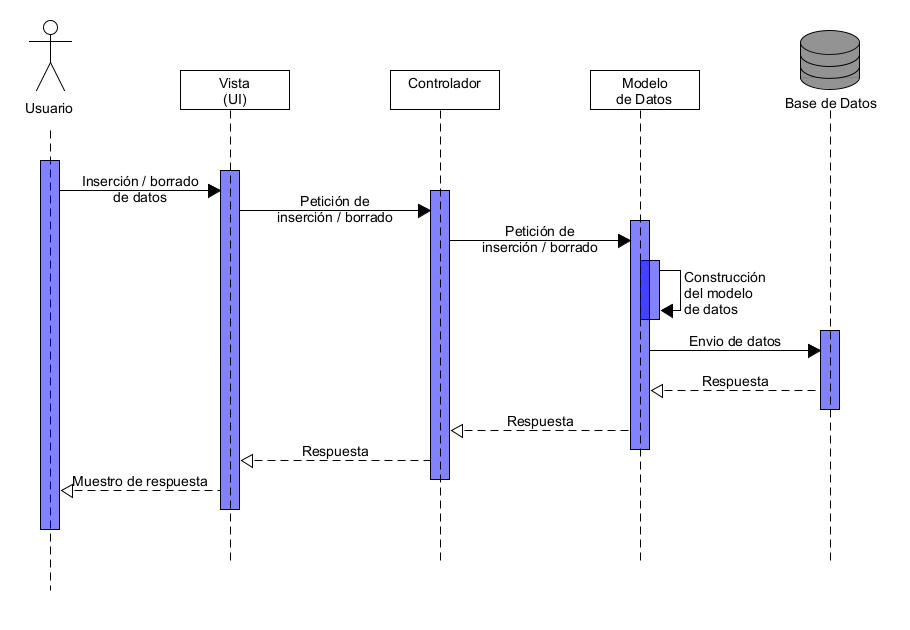
\includegraphics[scale=0.5]{img/imgs-memoria/Secuencias_Ins_DeL.png}
    \caption{Diagrama de secuencias de una inserción / borrado}
\end{figure}

Por último, en los siguientes diagramas se refleja el manejo de las acciones relacionadas con el autograding y generación de tareas mediante Nbgrader, acciones realizadas mediante la implementación de una clase de manejo (manager / gerente) de la API pública de esta herramienta:

\begin{figure}[H]
    \centering
    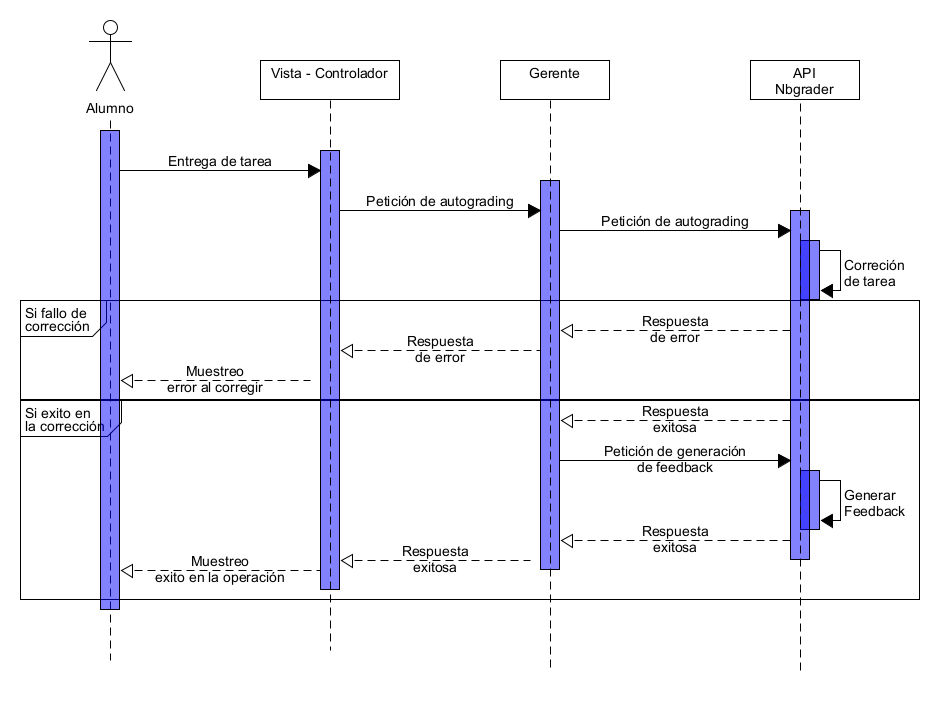
\includegraphics[width=\textwidth]{img/imgs-memoria/Secuencias_Autograding.png}
    \caption{Diagrama de secuencias autograding}
\end{figure}


\begin{figure}[H]
    \hspace*{-2cm} 
    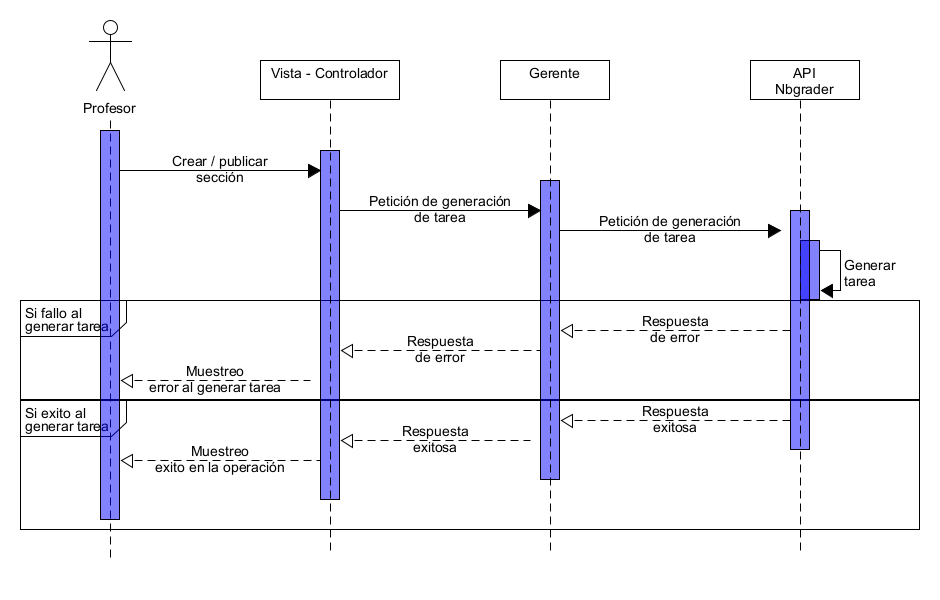
\includegraphics[scale=0.5]{img/imgs-memoria/Secuencias_Generate.png}
    \caption{Diagrama de secuencias generación de tarea}
\end{figure}


\section{Diseño arquitectónico}
Como ya se ha mencionado con anterioridad, el desarrollo de esta plataforma ha sido realizada mediante Flask. Flask es un framework minimalista no ligado a ningún diseño arquitectónico predefinido, lo cual ofrece a desarrolladores una gran libertad en cuanto a qué patrón arquitectónico dar a su proyecto.

En el caso de este proyecto, el patrón arquitectónico escogido ha sido \textbf{MVC (Modelo - Vista - Controlador)}:

\begin{figure}[H]
    \centering
    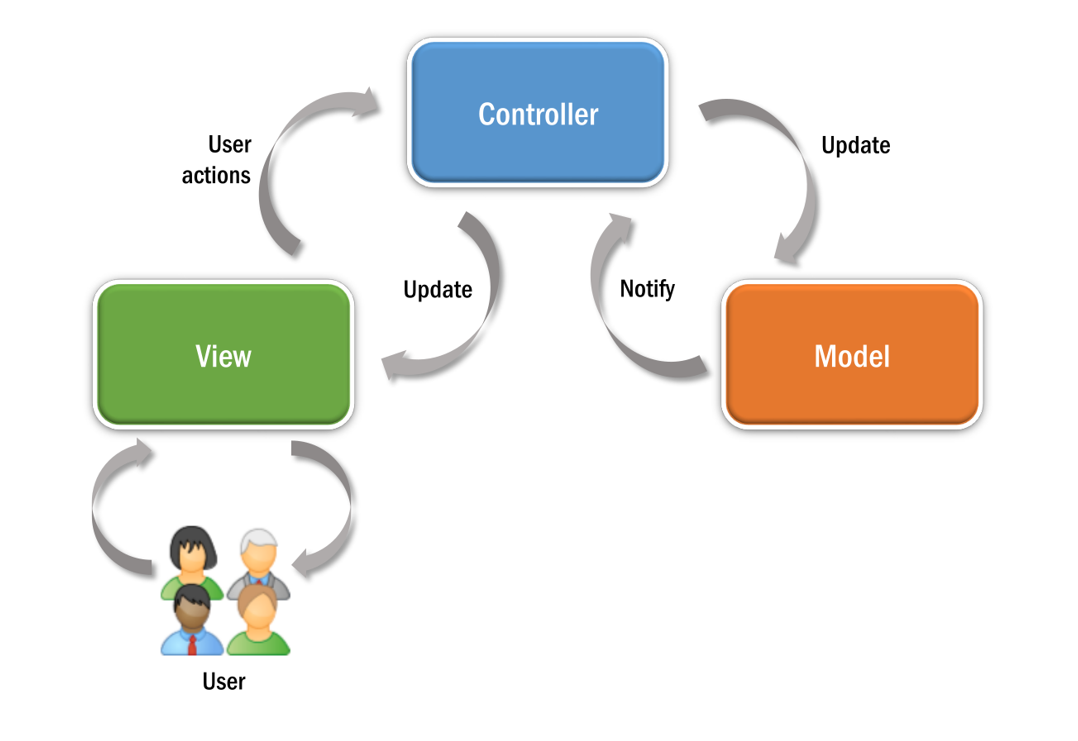
\includegraphics[scale=0.4]{img/imgs-memoria/MVC.png}
    \caption{Representación MVC}
\end{figure}

Este es un patrón software basado en la división de responsabilidades de una aplicación en tres capas diferentes:
\begin{itemize}
\item \textbf{Modelo:} Encargada de la representación y acceso a los datos del dominio junto con la lógica de negocio de estos.

\item \textbf{Vista:} Responsable de la generación de la interfaz de usuario, medio por el que los clientes visualizan la información e interactuan con el sistema.

\item \textbf{Controlador:} Intermediario entre las capas anteriores, encargado de gestionar el flujo de información entre las mismas.

\end{itemize}

En lo que a nuestro proyecto respecta, los métodos ruta o endpoints, que desempeñan la labor de Controlador, se encuentran en el fichero \textbf{routes.py}. La capa de Vista queda constituida por los directorios \textbf{templates} y \textbf{static} en los que se encuentran los documentos html, estilos e imágenes que componen la aplicación. La función de renderizado de vistas es desempeñada por el motor de templates Jinja2 sobre el que Flask está montado. Finalmente Flask no tiene predifinido ningún ORM (Asignación objeto-relacional) encargado de la función de Modelo y por ello la herramienta seleccionada para esta función es la mencionada con anteriordad SQLAlchemy.




